\documentclass[11pt,a4paper]{article}
\usepackage[utf8]{inputenc}
\usepackage[T1]{fontenc}
\usepackage[spanish,provide=*]{babel}
\usepackage{lmodern,amsmath,amssymb,graphicx,microtype}
\usepackage[margin=24mm]{geometry}
\usepackage{xcolor,float,fancyhdr,needspace,etoolbox}
\definecolor{deepgreen}{HTML}{174B37}
\usepackage[colorlinks=true,linkcolor=deepgreen,urlcolor=deepgreen]{hyperref}
\floatplacement{figure}{H}
\providecommand{\tightlist}{\setlength{\itemsep}{0pt}\setlength{\parskip}{0pt}}
\setlength{\parindent}{0pt}\setlength{\parskip}{5pt}
\setlength{\emergencystretch}{3em}
\pagestyle{fancy}\fancyhf{}
\fancyhead[L]{\small Métodos Matemáticos para las Ciencias}
\fancyhead[R]{\small Capítulo 2}
\fancyfoot[C]{\thepage}\setlength{\headheight}{14pt}
\setcounter{secnumdepth}{0}\setcounter{tocdepth}{1}
\pretocmd{\section}{\needspace{5\baselineskip}}{}{}
\pretocmd{\subsection}{\needspace{4\baselineskip}}{}{}
\begin{document}
\begin{center}
{\color{deepgreen}\Huge\bfseries Ecuaciones de transporte}\par\vspace{6mm}
{\Large Capítulo 2 · Notas de clase}\par\vspace{5mm}
Lourival Rodrigues de Lima\par
Métodos Matemáticos para las Ciencias · MATG1075 · ESPOL
\end{center}
\vspace{5mm}
Basadas en el capítulo 2 de T. Witelski y M. Bowen (2015). Se mantienen los temas, ejemplos y símbolos del libro. Las notas de revisión señalan erratas del original. La versión web contiene tres figuras interactivas; aquí se presentan sus versiones estáticas.
\tableofcontents\newpage
\hypertarget{introducciuxf3n-del-individuo-al-continuo}{%
\section{Introducción: del individuo al
continuo}\label{introducciuxf3n-del-individuo-al-continuo}}

En el capítulo anterior, las variables dependían principalmente del
tiempo. Ahora una propiedad también puede variar con la posición:
escribimos \(\rho(x,t)\) o, en varias dimensiones,
\(\rho(\mathbf x,t)\). El objetivo es describir cómo se redistribuye una
cantidad cuando hay movimiento, producción o pérdida.

La \textbf{hipótesis del continuo} reemplaza el seguimiento de
individuos por campos promediados sobre regiones pequeñas. La densidad
\(f(x,t)\) representa cantidad por unidad de longitud, área o volumen,
según el modelo. Su integral es una cantidad total:

\[F(t)=\int f(x,t)\,dx.\]

La variable espacial puede representar una posición física, pero también
edad, tamaño u otra característica de una población. Por ello, las
ecuaciones de transporte aparecen en fluidos, sólidos, poblaciones
estructuradas y otros sistemas.

Estas notas desarrollan, con redacción propia, el capítulo 2 de Witelski
y Bowen (2015), pp.~23--45. Las secciones 2.1--2.6 contienen la teoría;
2.7 orienta lecturas y 2.8 organiza los ejercicios del libro. Se
mantienen las variables y la numeración de las ecuaciones citadas del
libro. Las figuras interactivas corresponden a sus ejemplos de
características y de Burgers. Se supone suficiente regularidad cuando se
derivan identidades punto a punto; al aparecer choques se vuelve a la
formulación integral.

\hypertarget{teorema-de-transporte-de-reynolds}{%
\section{2.1. Teorema de transporte de
Reynolds}\label{teorema-de-transporte-de-reynolds}}

\hypertarget{dos-descripciones-del-movimiento}{%
\subsection{Dos descripciones del
movimiento}\label{dos-descripciones-del-movimiento}}

Una \textbf{descripción euleriana} especifica campos en posiciones
fijas, por ejemplo la velocidad \(\mathbf v(\mathbf x,t)\). Una
\textbf{descripción lagrangiana} sigue una partícula etiquetada por su
posición inicial \(\mathbf A\). Su trayectoria satisface

\[\frac{d\mathbf X}{dt}=\mathbf v(\mathbf X(t;\mathbf A),t),\qquad \mathbf X(0;\mathbf A)=\mathbf A.\]

Si \(f(\mathbf x,t)\) es una propiedad, su valor sobre esa trayectoria
es \(F(t;\mathbf A)=f(\mathbf X(t;\mathbf A),t)\) (2.4). La velocidad
lagrangiana es
\(\mathbf V(t;\mathbf A)=\mathbf v(\mathbf X(t;\mathbf A),t)\) (2.2). La
regla de la cadena da

\[\frac{df_{\mathrm{part}}}{dt}=\frac{\partial f}{\partial t}+\mathbf v\cdot\nabla f\equiv\frac{Df}{Dt}.\tag{2.5}\]

Aquí \(f_{\mathrm{part}}(t)\equiv F(t;\mathbf A)\).

El operador \(D/Dt\) es la \textbf{derivada material o convectiva}. En
una dimensión es \(\partial_t+v\partial_x\). No se confunde con
\(\partial_t\): esta última observa un lugar fijo, mientras que la
derivada material acompaña una partícula.

Si la velocidad está prescrita, estudiamos un problema cinemático. Si
depende de las propiedades que buscamos y debe determinarse con ellas,
el problema es dinámico. En el transporte pasivo, la sustancia
transportada no modifica el campo de velocidad.

\hypertarget{un-intervalo-que-se-mueve-con-el-flujo}{%
\subsection{Un intervalo que se mueve con el
flujo}\label{un-intervalo-que-se-mueve-con-el-flujo}}

El libro denota por \(f_{\mathrm{blob}}\) la cantidad acumulada sobre un
dominio material:

\[f_{\mathrm{blob}}(t)=\iiint_{D(t)}f(\mathbf x,t)\,dV,\tag{2.6}\]

y, en una dimensión,

\[f_{\mathrm{blob}}(t)=\int_{a(t)}^{b(t)}f(x,t)\,dx.\tag{2.7}\]

Sea \([a(t),b(t)]\) un intervalo material: \(a'=v(a,t)\) y
\(b'=v(b,t)\). Por la regla de Leibniz,

\[\begin{aligned}
\frac{d}{dt}\int_{a(t)}^{b(t)} f(x,t)\,dx
&=\int_a^b f_t\,dx+f(b,t)b'-f(a,t)a'\\
&=\int_a^b\left[f_t+(fv)_x\right]\,dx.
\end{aligned}\tag{2.8}\]

Los términos de los extremos contabilizan el movimiento del intervalo.
Omitirlos equivale a tratar como fijo un dominio que no lo es.

\hypertarget{forma-multidimensional}{%
\subsection{Forma multidimensional}\label{forma-multidimensional}}

Para un dominio material \(D(t)\) cuya frontera se mueve con
\(\mathbf v\), el \textbf{teorema de transporte de Reynolds} establece

\[\boxed{\frac{d}{dt}\int_{D(t)} f\,dV=\int_{D(t)}\bigl[\partial_t f+\nabla\cdot(f\mathbf v)\bigr]\,dV.}\tag{2.9}\]

Equivalentemente, el integrando es \(Df/Dt+f\nabla\cdot\mathbf v\). El
segundo término mide el efecto de la expansión o contracción del
volumen. El teorema también se obtiene sumando la variación local y el
flujo debido a la frontera móvil, y aplicando el teorema de la
divergencia.

\hypertarget{deducciuxf3n-de-leyes-de-conservaciuxf3n}{%
\section{2.2. Deducción de leyes de
conservación}\label{deducciuxf3n-de-leyes-de-conservaciuxf3n}}

\hypertarget{de-una-identidad-integral-a-una-ecuaciuxf3n-local}{%
\subsection{De una identidad integral a una ecuación
local}\label{de-una-identidad-integral-a-una-ecuaciuxf3n-local}}

Si una función continua \(g\) tiene integral cero en \textbf{todo}
subintervalo, entonces \(g=0\). En efecto, si \(g(x_0)>0\), la
continuidad proporciona un intervalo donde \(g>0\), cuya integral sería
positiva; el caso negativo es análogo. La condición «todo subdominio» es
esencial.

Supongamos que la masa de cada dominio material permanece constante.
Reynolds implica

\[0=\int_{D(t)}\bigl[\rho_t+\nabla\cdot(\rho\mathbf v)\bigr]\,dV.\]

Como vale para cualquier dominio material, obtenemos la \textbf{ecuación
de continuidad}:

\[\boxed{\rho_t+\nabla\cdot(\rho\mathbf v)=0.}\tag{2.13}\]

En una dimensión, \(\rho_t+(\rho v)_x=0\). El flujo es \(q=\rho v\):
cantidad que cruza una sección por unidad de tiempo. En varias
dimensiones, \(\rho\mathbf v\cdot\mathbf n\) es el flujo normal por
unidad de área, con \(\mathbf n\) normal exterior.

Expandiendo la divergencia,

\[\frac{D\rho}{Dt}=-\rho\nabla\cdot\mathbf v.\]

\textbf{Conservar masa no significa conservar densidad sobre una
trayectoria.} Si el volumen se expande, la densidad disminuye. Solo para
un flujo sin divergencia, y sin fuentes, se obtiene \(D\rho/Dt=0\).

\hypertarget{fuentes-y-sumideros}{%
\subsection{Fuentes y sumideros}\label{fuentes-y-sumideros}}

Sea \(R\) la producción neta por unidad de volumen y tiempo. Si

\[\frac{d}{dt}\int_{D(t)}\rho\,dV=\int_{D(t)}R\,dV,\]

entonces

\[\rho_t+\nabla\cdot(\rho\mathbf v)=R,\qquad \frac{D\rho}{Dt}=R-\rho\nabla\cdot\mathbf v.\]

En un intervalo \textbf{fijo} \([a,b]\), el balance es

\[\frac{d}{dt}\int_a^b\rho\,dx=q(a,t)-q(b,t)+\int_a^b R\,dx.\]

Así, el total cambia por entrada menos salida, más producción interna.

\hypertarget{conservaciuxf3n-del-momento}{%
\subsection{Conservación del
momento}\label{conservaciuxf3n-del-momento}}

El momento por unidad de volumen es \(\rho\mathbf v\). Aplicar Reynolds
componente a componente y la segunda ley de Newton conduce a

\[\frac{\partial(\rho\mathbf v)}{\partial t}+\nabla\cdot(\rho\mathbf v\mathbf v)=\nabla\cdot\boldsymbol\sigma.\tag{2.18}\]

Aquí \(\boldsymbol\sigma\) es el tensor de esfuerzos;
\(\mathbf v\mathbf v\) es el producto diádico, con componentes
\(v_i v_j\). El libro escribe la fuerza por unidad de volumen como
\(\mathbf f=\nabla\cdot\boldsymbol\sigma\). Esta expresión considera
fuerzas representadas por esfuerzos, como en el capítulo. Junto con
continuidad, equivale a
\(\rho D\mathbf v/Dt=\nabla\cdot\boldsymbol\sigma\). Para cerrar un
modelo deben especificarse relaciones constitutivas que expresen los
esfuerzos en función de las variables del sistema.

\hypertarget{ecuaciuxf3n-de-advecciuxf3n-lineal}{%
\section{2.3. Ecuación de advección
lineal}\label{ecuaciuxf3n-de-advecciuxf3n-lineal}}

Sin fuentes y con velocidad constante \(c\), la continuidad se reduce a

\[\rho_t+c\rho_x=0,\qquad \rho(x,0)=P(x),\quad x\in\mathbb R.\]

La solución es

\[\boxed{\rho(x,t)=P(x-ct).}\tag{2.20}\]

Para verificarlo, \(\rho_t=-cP'(x-ct)\) y \(\rho_x=P'(x-ct)\). El perfil
se traslada sin deformarse: hacia la derecha si \(c>0\), hacia la
izquierda si \(c<0\), y permanece fijo si \(c=0\). Cada característica
es \(x=A+ct\) y transporta el valor \(P(A)\).

\hypertarget{modos-de-fourier-y-relaciuxf3n-de-dispersiuxf3n}{%
\subsection{Modos de Fourier y relación de
dispersión}\label{modos-de-fourier-y-relaciuxf3n-de-dispersiuxf3n}}

El libro escribe el perfil mediante su serie compleja de Fourier,
\(P(x)=\sum_k A_ke^{ikx}\). Así, la onda viajera se expresa como

\[\rho(x,t)=\sum_{k=-\infty}^{\infty}A_ke^{ik(x-ct)}=\sum_{k=-\infty}^{\infty}A_ke^{i[kx-\omega t]}.\tag{2.21}\]
Para un modo

\[\rho_k(x,t)=A_k e^{i(kx-\omega t)},\]

\(k\) es el número de onda, \(\omega\) la frecuencia angular, y
\(\omega=\omega(k)\) la \textbf{relación de dispersión}. Para un modo
oscilatorio real con \(k\ne0\), la longitud de onda se denota \(L\) y el
período \(T\). El libro escribe \(L=2\pi/k\) y \(T=2\pi/\omega\),
tomando números de onda y frecuencias positivos para estas magnitudes.
Se toma la parte real para representar una magnitud real.

Al sustituir en advección resulta \(\omega=ck\). La velocidad de fase
\(c_p=\omega/k\) es la misma para todos los modos: no hay dispersión.

En cambio, para

\[\rho_t+c_1\rho_x+c_3\rho_{xxx}+c_5\rho_{xxxxx}=0,\tag{2.22}\]

la sustitución produce

\[-i\omega+ic_1k-ic_3k^3+ic_5k^5=0,\]

por lo que \(\omega=c_1k-c_3k^3+c_5k^5\) y \(c_p=c_1-c_3k^2+c_5k^4\). Al
propagarse los modos con velocidades distintas, su suma cambia de forma.

El libro también considera la difusión \(\rho_t=\rho_{xx}\). Sustituir
el mismo modo da \(\omega=-ik^2\), de manera que

\[\rho_k(x,t)=(A_k e^{-k^2t})e^{ikx}.\]

La amplitud decae y no hay propagación de fase. Así se distingue este
comportamiento de la dispersión, donde los modos pueden conservar
amplitud y desplazarse a velocidades diferentes.

\hypertarget{sistemas-de-advecciuxf3n-lineal}{%
\section{2.4. Sistemas de advección
lineal}\label{sistemas-de-advecciuxf3n-lineal}}

El libro considera dos propiedades \(p(x,t)\) y \(q(x,t)\) sobre
\(-\infty<x<\infty\), con coeficientes constantes:

\[p_t+ap_x+bq_x=0,\tag{2.23a}\] \[q_t+cp_x+dq_x=0,\tag{2.23b}\]
\[p(x,0)=f(x),\qquad q(x,0)=g(x).\tag{2.23c}\]

Buscamos una variable que obedezca una ecuación de advección
independiente:

\[w_t+\lambda w_x=0\quad\Longrightarrow\quad w(x,t)=W(x-\lambda t).\tag{2.24}\]

Para ello se propone la combinación

\[w(x,t)=Ap(x,t)+Bq(x,t),\tag{2.25}\]

con \(A,B\) constantes por determinar. Multiplicar (2.23a) por \(A\) y
(2.23b) por \(B\) y sumar produce

\[(Ap+Bq)_t+(aA+cB)p_x+(bA+dB)q_x=0.\]

Comparar con \(w_t+\lambda w_x=0\) da

\[\begin{pmatrix}a&c\\b&d\end{pmatrix}\begin{pmatrix}A\\B\end{pmatrix}=\lambda\begin{pmatrix}A\\B\end{pmatrix}.\tag{2.26}\]

Los valores propios determinan las velocidades. Dos vectores propios
independientes dan las relaciones

\[\begin{aligned}
w_1(x,t)&=A_1p(x,t)+B_1q(x,t)=W_1(x-\lambda_1t),\\
w_2(x,t)&=A_2p(x,t)+B_2q(x,t)=W_2(x-\lambda_2t).
\end{aligned}\tag{2.27}\]

Las condiciones iniciales fijan los perfiles:

\[A_1f(x)+B_1g(x)=W_1(x),\qquad A_2f(x)+B_2g(x)=W_2(x).\tag{2.28}\]

Conocidos los lados derechos de (2.27), se resuelve ese sistema
algebraico para recuperar \(p\) y \(q\).

Para \(n\) ecuaciones, el libro utiliza \(\mathbf p=(p,q,r,\ldots)^T\):

\[\frac{\partial\mathbf p}{\partial t}+M\frac{\partial\mathbf p}{\partial x}=0.\tag{2.29}\]

Se propone \(w=\mathbf u\cdot\mathbf p\), con
\(\mathbf u=(A,B,C,\ldots)^T\), y se obtiene

\[M^T\mathbf u=\lambda\mathbf u.\tag{2.30}\]

Si todos los valores propios son reales y existe una base completa de
vectores propios, el sistema se denomina \textbf{hiperbólico}, en el
sentido utilizado en el capítulo. Entonces sus soluciones se expresan
mediante sumas de ondas viajeras. Los símbolos \(A,B\) de esta sección
son coeficientes de una combinación lineal; en la sección siguiente,
\(A\) vuelve a representar la posición inicial de una característica.

\hypertarget{muxe9todo-de-las-caracteruxedsticas}{%
\section{2.5. Método de las
características}\label{muxe9todo-de-las-caracteruxedsticas}}

Una ecuación semilineal de primer orden tiene la forma

\[p_t+c(x,t)p_x=r(x,t,p),\qquad p(x,0)=f(x).\]

La velocidad no depende de \(p\), aunque la reacción sí puede hacerlo.
Definimos \(P(t;A)=p(X(t;A),t)\). La regla de la cadena convierte la EDP
en el sistema

\[\boxed{X'=c(X,t),\quad P'=r(X,t,P),\quad X(0;A)=A,\quad P(0;A)=f(A).}\]

El procedimiento consiste en resolver \(X\), resolver después \(P\) y,
si es posible, invertir \(x=X(t;A)\) para recuperar la etiqueta
\(A=A(x,t)\). Finalmente, \(p(x,t)=P(t;A(x,t))\).

\hypertarget{ejemplo-del-capuxedtulo}{%
\subsection{Ejemplo del capítulo}\label{ejemplo-del-capuxedtulo}}

Para

\[p_t+2xp_x=xp^2,\qquad p(x,0)=2+\sin x,\tag{2.35}\]

las características satisfacen \(X'=2X\), de modo que \(X=Ae^{2t}\).
Entonces

\[P'=Ae^{2t}P^2,\qquad \frac{d}{dt}\left(\frac1P\right)=-Ae^{2t}.\]

Integrando y usando el dato inicial,

\[P(t;A)=\left[\frac{1}{2+\sin A}-\frac A2(e^{2t}-1)\right]^{-1}.\]

Como \(A=xe^{-2t}\), obtenemos

\[\boxed{p(x,t)=\left[\frac{1}{2+\sin(xe^{-2t})}+\frac x2(e^{-2t}-1)\right]^{-1}.}\]

La expresión es válida donde la solución permanece finita y el cambio de
variables puede invertirse. En la figura se evita el denominador cero.

\begin{figure}
\centering
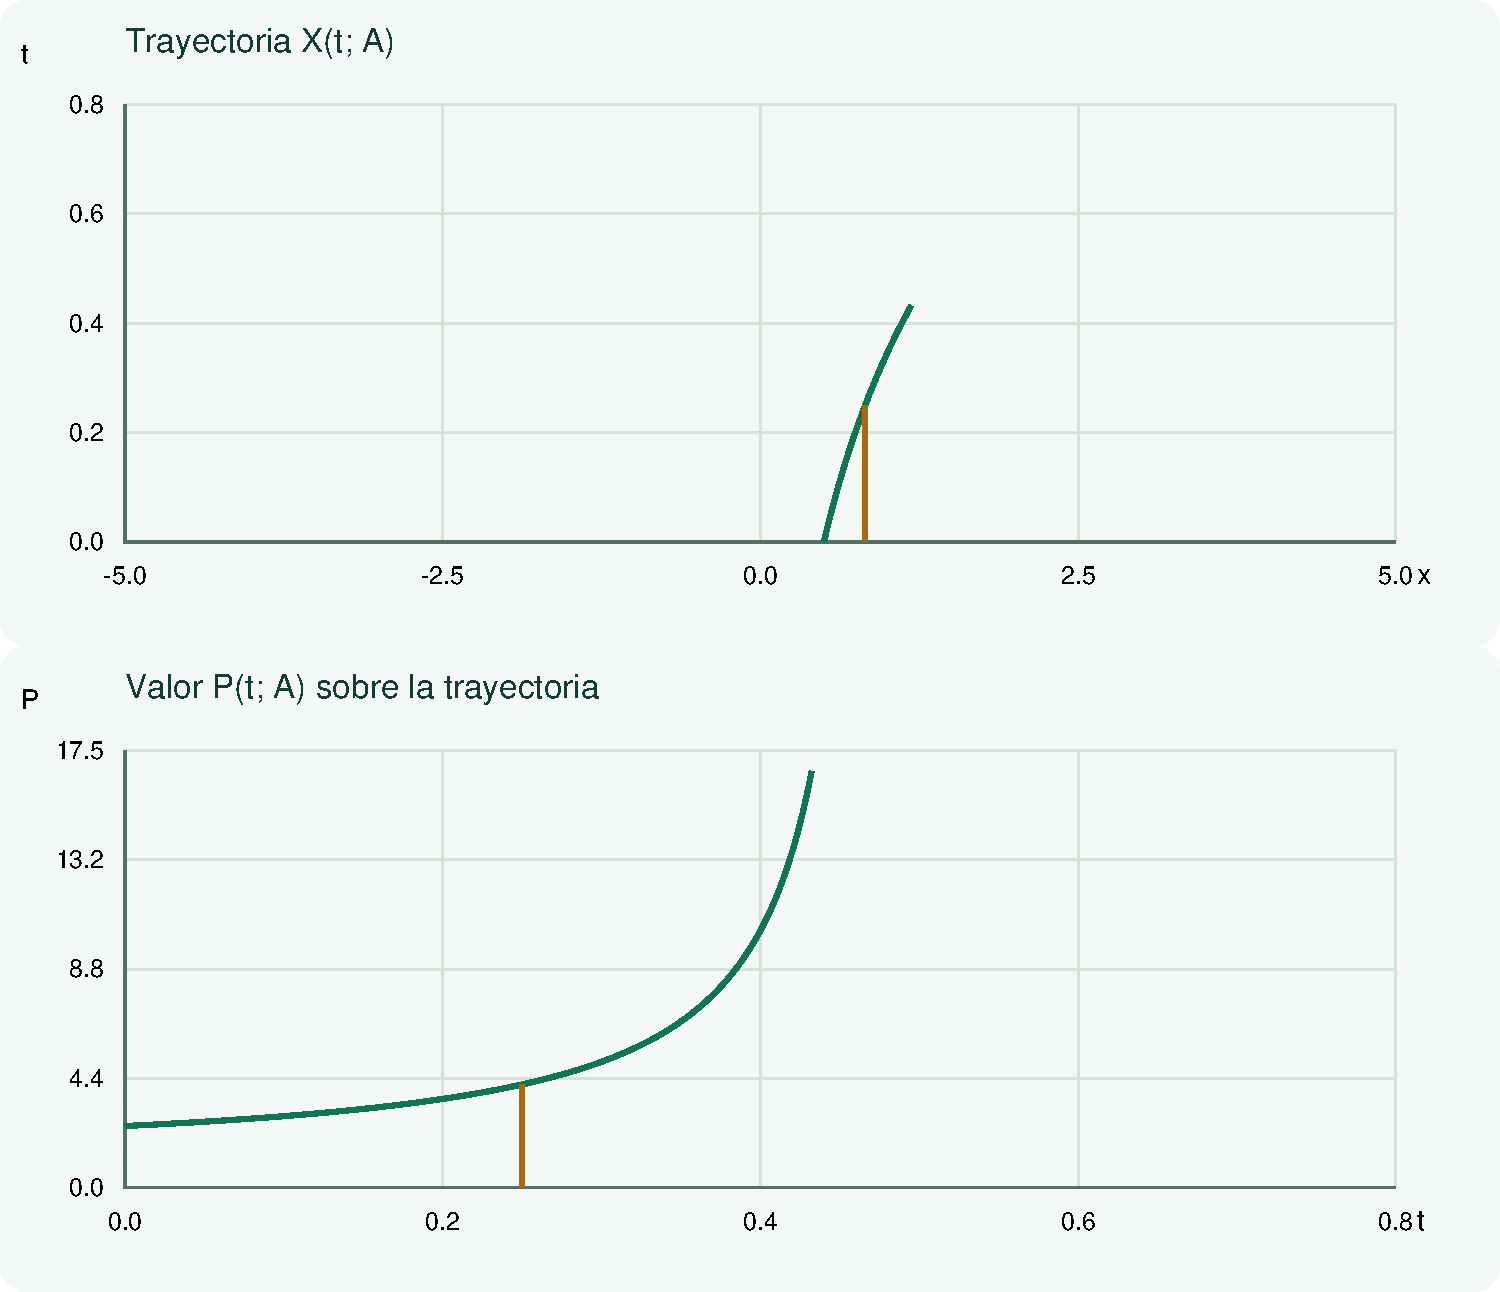
\includegraphics[width=0.78\textwidth]{characteristic.pdf}
\caption{Trayectoria y valor de la solución sobre una característica
seleccionada. La visualización no prolonga la fórmula a través de una
explosión.}
\end{figure}

\hypertarget{choques-en-ecuaciones-cuasilineales}{%
\section{2.6. Choques en ecuaciones
cuasilineales}\label{choques-en-ecuaciones-cuasilineales}}

\hypertarget{cuando-la-velocidad-depende-de-la-soluciuxf3n}{%
\subsection{Cuando la velocidad depende de la
solución}\label{cuando-la-velocidad-depende-de-la-soluciuxf3n}}

Para \(p_t+c(x,t,p)p_x=r(x,t,p)\), las ecuaciones características son
\(X'=c(X,t,P)\) y \(P'=r(X,t,P)\). Ahora están acopladas. Dos
características con valores distintos pueden alcanzar el mismo punto: la
representación paramétrica deja de definir una función univaluada.

La ecuación de Burgers sin viscosidad es

\[p_t+pp_x=0,\qquad p(x,0)=f(x).\]

Sus características satisfacen

\[P(t;A)=f(A),\qquad X(t;A)=A+tf(A).\]

\hypertarget{pulso-triangular-del-capuxedtulo}{%
\subsection{Pulso triangular del
capítulo}\label{pulso-triangular-del-capuxedtulo}}

Consideremos \(f(A)=\max(1-|A|,0)\). Las cuatro ramas características
son

\[\begin{cases}
X=A,\quad P=0,&A<-1,\\
X=(1+A)t+A,\quad P=1+A,&-1\le A\le0,\\
X=(1-A)t+A,\quad P=1-A,&0\le A\le1,\\
X=A,\quad P=0,&A>1.
\end{cases}\tag{2.42}\]

Para \(0\le t<1\),

\[p(x,t)=\begin{cases}
0,&x<-1,\\
\dfrac{1+x}{1+t},&-1\le x\le t,\\
\dfrac{1-x}{1-t},&t<x\le1,\\
0,&x>1.
\end{cases}\tag{2.43}\]

La rama izquierda se expande; la derecha se comprime. El perfil es
continuo y suave por tramos, no globalmente diferenciable en sus
esquinas. En \(t=1\), todas las características de \(0\le A\le1\)
alcanzan \(x=1\). Prolongarlas más allá produciría valores múltiples. La
solución física se construye con un salto móvil o \textbf{choque}.

\begin{figure}
\centering
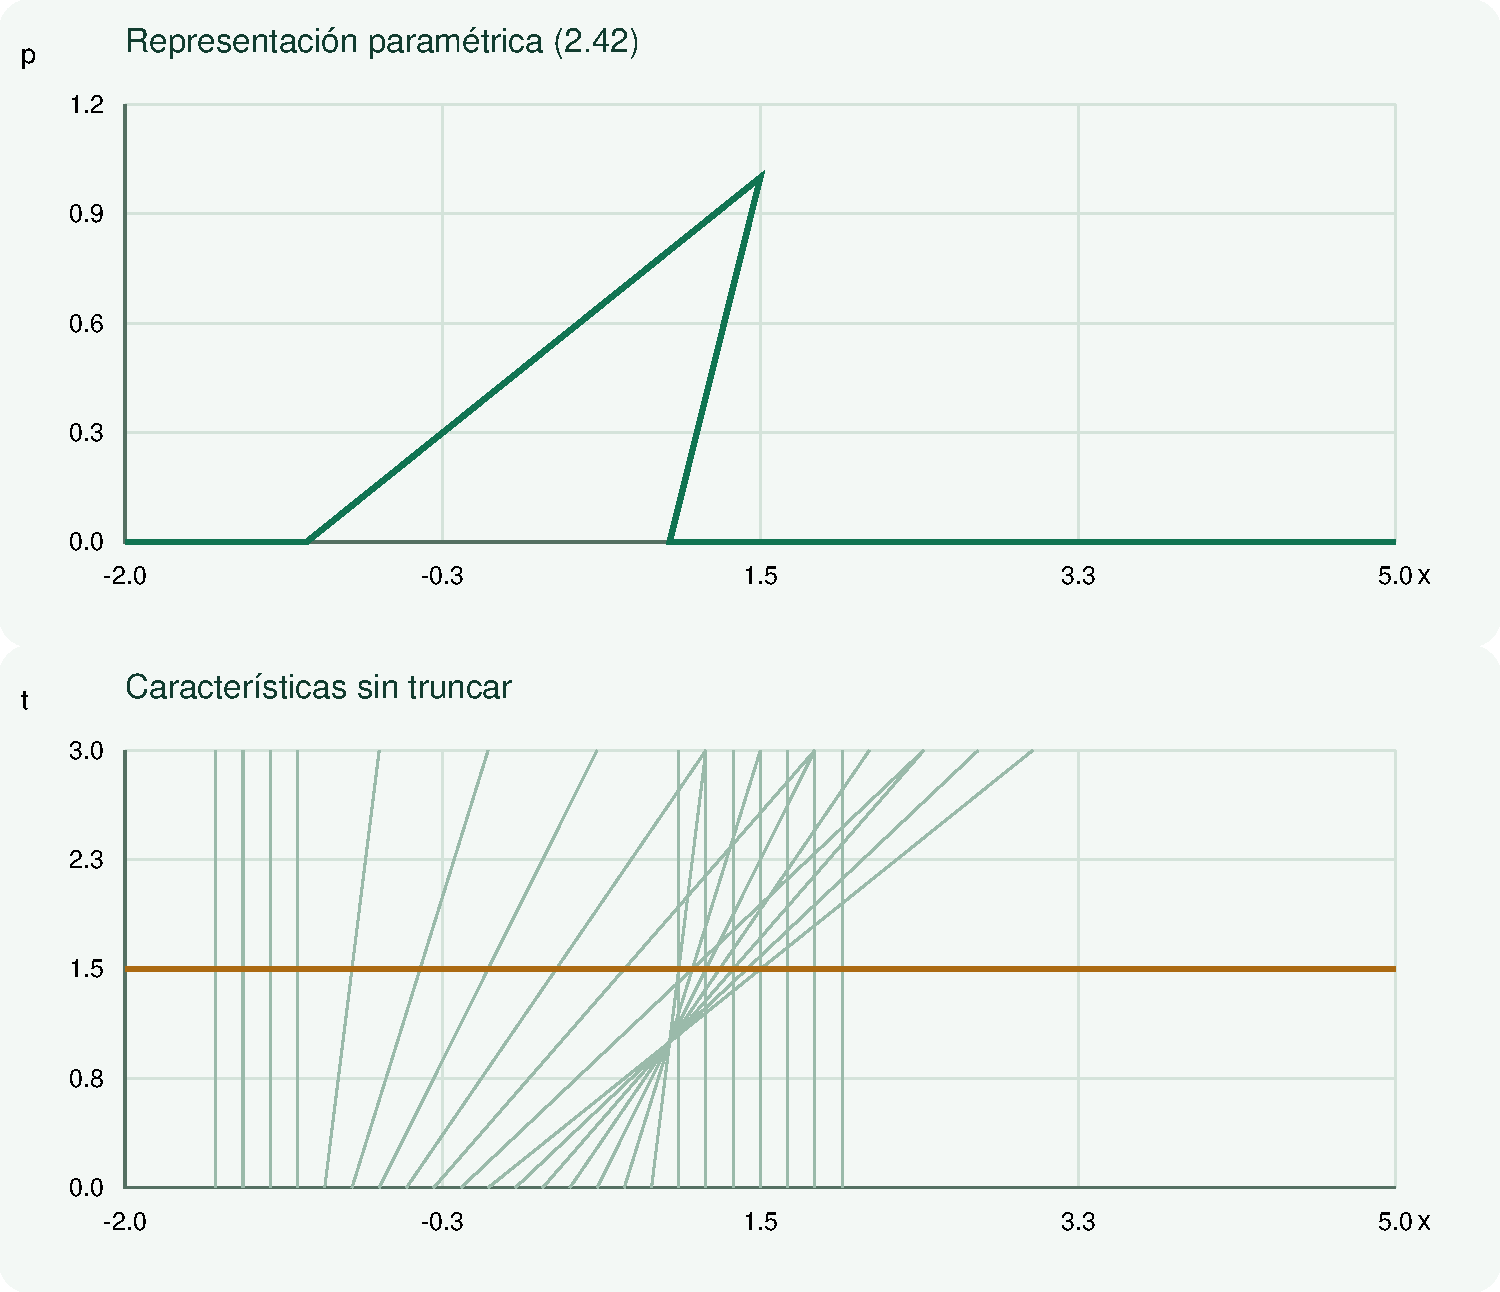
\includegraphics[width=0.78\textwidth]{breaking.pdf}
\caption{Ejemplo (2.40)--(2.43): características y representación
paramétrica del pulso triangular. Después de t = 1, las ramas
superpuestas todavía no constituyen una solución univaluada.}
\end{figure}

\hypertarget{balance-integral-y-condiciuxf3n-de-rankinehugoniot}{%
\subsection{Balance integral y condición de
Rankine--Hugoniot}\label{balance-integral-y-condiciuxf3n-de-rankinehugoniot}}

Escribamos la ley conservativa como \(p_t+\partial_x q(p)=0\). En un
intervalo fijo,

\[\frac{d}{dt}\int_a^b p\,dx=q(p(a,t))-q(p(b,t)).\]

Sea \(x_s(t)\) la posición de un salto, con valores laterales \(p_-\) a
la izquierda y \(p_+\) a la derecha. Dividimos la integral en
\([a,x_s(t)]\) y \([x_s(t),b]\). Leibniz aporta el término
\(x_s'(p_--p_+)\); los flujos interiores aportan \(q(p_+)-q(p_-)\). Su
suma debe ser cero, y resulta

\[\frac{dx_s}{dt}=\frac{q(p_+(x_s,t))-q(p_-(x_s,t))}{p_+(x_s,t)-p_-(x_s,t)}.\tag{2.48}\]

Se supone que los estados laterales son distintos.

Esta condición expresa conservación a través del salto y determina su
velocidad una vez conocidos los estados laterales.

Para Burgers, \(q(p)=p^2/2\), así que

\[\boxed{x_s'=\frac{p_-+p_+}{2}.}\]

\textbf{Nota de revisión del texto.} En la primera igualdad de (2.49),
p.~37, el libro imprime una diferencia entre los estados. La
factorización en (2.48) da la suma \((p_++p_-)/2\), coherente con la
segunda igualdad de (2.49). Aquí se conserva la notación y se corrige
explícitamente ese signo.

\hypertarget{soluciuxf3n-despuuxe9s-del-choque}{%
\subsection{Solución después del
choque}\label{soluciuxf3n-despuuxe9s-del-choque}}

En el pulso triangular, \(p_-=(1+x_s)/(1+t)\) y \(p_+=0\). Por tanto,

\[x_s'=\frac{1+x_s}{2(1+t)},\qquad x_s(1)=1.\]

Separando variables, \(\log(1+x_s)=\tfrac12\log(1+t)+C\). La condición
inicial fija la constante y obtenemos

\[x_s(t)=\sqrt{2(1+t)}-1,\qquad t\ge1.\]

La solución conservativa para \(t\ge1\) es

\[p(x,t)=\begin{cases}\dfrac{1+x}{1+t},&-1\le x<x_s(t),\\0,&x<-1\ \text{o}\ x>x_s(t).\end{cases}\]

El valor asignado exactamente en el salto no altera las integrales. La
altura izquierda es \(p_- =\sqrt{2/(1+t)}\). El área se conserva:

\[\int_{\mathbb R}p(x,t)\,dx=\frac12\underbrace{\sqrt{2(1+t)}}_{\text{base}}\underbrace{\sqrt{2/(1+t)}}_{\text{altura}}=1.\]

La construcción elimina las ramas superpuestas respetando el balance de
área. Esta selección también se describe en el libro como regla de áreas
iguales.

\begin{figure}
\centering
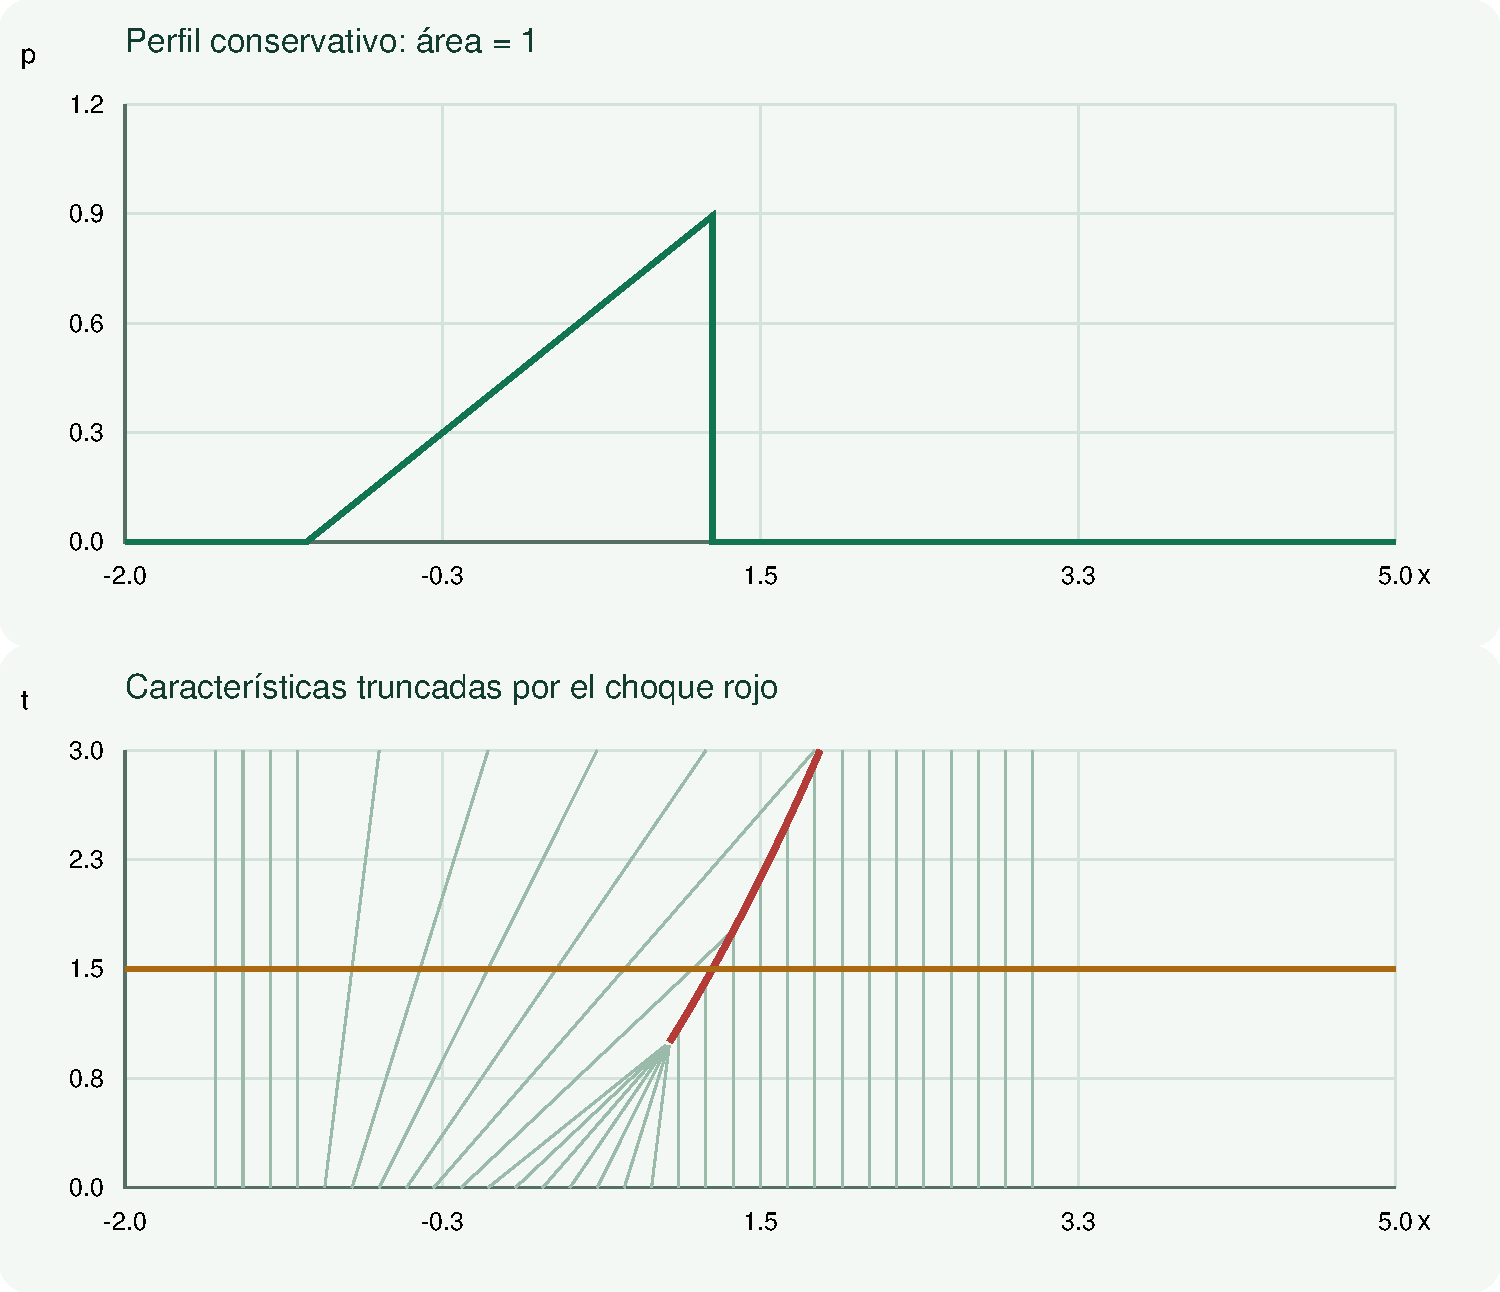
\includegraphics[width=0.78\textwidth]{shock.pdf}
\caption{Formación del choque en el pulso triangular. El perfil conserva
área uno antes y después del tiempo crítico t = 1; la curva roja
representa el choque.}
\end{figure}

\hypertarget{para-continuar-la-lectura}{%
\section{2.7. Para continuar la
lectura}\label{para-continuar-la-lectura}}

El capítulo remite a textos sobre ondas lineales y no lineales y a
tratamientos de EDP que desarrollan las características. Antes de
avanzar, conviene poder distinguir: descripción euleriana y lagrangiana;
derivada parcial y material; advección y conservación con velocidad
variable; dispersión y disipación; solución clásica y solución con
choque.

\textbf{Referencia principal:} T. Witelski y M. Bowen, \emph{Methods of
Mathematical Modelling: Continuous Systems and Differential Equations},
Springer, 2015, capítulo 2, «Transport Equations», pp.~23--45. Estas
notas son material de apoyo y deben utilizarse junto con el libro y las
indicaciones de clase.

\hypertarget{ejercicios}{%
\section{2.8. Ejercicios}\label{ejercicios}}

Los ejercicios siguientes corresponden a los problemas 2.1--2.15 del
capítulo. Se conservan sus datos y notación, con enunciados reformulados
en español. No se añaden problemas externos ni soluciones a esta
sección.

\hypertarget{promedio-sobre-un-intervalo-material}{%
\subsection{2.1. Promedio sobre un intervalo
material}\label{promedio-sobre-un-intervalo-material}}

Los extremos \(a(t)\) y \(b(t)\) se mueven según \(dx/dt=v(x,t)\). Para

\[f_{\mathrm{avg}}(t)=\frac{1}{b(t)-a(t)}\int_{a(t)}^{b(t)}f(x,t)\,dx,\]

calcular \(\lim_{b\to a}df_{\mathrm{avg}}/dt\). Utilizar
\(b(t)=a(t)+\varepsilon h(t)\) con \(\varepsilon\to0\).

\hypertarget{momento-de-un-gas-compresible}{%
\subsection{2.2. Momento de un gas
compresible}\label{momento-de-un-gas-compresible}}

Partiendo de

\[\rho_t+(\rho v)_x=0,\qquad \rho(v_t+vv_x)=-P_x,\]

demostrar la equivalencia de la segunda ecuación con

\[(\rho v)_t+(\rho v^2)_x=-P_x.\]

Aquí \(P(x,t)\) es la presión y \(\rho Dv/Dt\) expresa la aceleración
material multiplicada por la densidad.

\hypertarget{velocidades-de-fase-y-de-grupo}{%
\subsection{2.3. Velocidades de fase y de
grupo}\label{velocidades-de-fase-y-de-grupo}}

Considerar

\[\rho(x,t)=\cos(kx-\omega(k)t)+\cos([k+\varepsilon]x-\omega(k+\varepsilon)t).\]

\begin{enumerate}
\def\labelenumi{(\alph{enumi})}
\tightlist
\item
  Para \(\varepsilon\to0\), reescribir la suma en la forma
\end{enumerate}

\[\rho(x,t)=2\cos(k[x-c_p(k)t])\cos\!\left(\tfrac12\varepsilon[x-c_g(k)t]\right)+O(\varepsilon),\]

e identificar la velocidad de grupo \(c_g\).

\begin{enumerate}
\def\labelenumi{(\alph{enumi})}
\setcounter{enumi}{1}
\tightlist
\item
  Para
\end{enumerate}

\[\rho_t+\rho_x-\rho_{xxt}=0,\tag{2.51}\]

obtener la relación de dispersión mediante \(\rho=\cos(kx-\omega t)\) y
calcular \(c_g\). Determinar también la relación modificada
\(\widetilde\omega(k)\) utilizando \(\rho=e^{kx-\widetilde\omega t}\).

\hypertarget{ondas-solitarias}{%
\subsection{2.4. Ondas solitarias}\label{ondas-solitarias}}

Para la ecuación de Benjamin--Bona--Mahony,

\[\rho_t+\rho_x+6\rho\rho_x-\rho_{xxt}=0,\]

\begin{enumerate}
\def\labelenumi{(\alph{enumi})}
\item
  introducir \(\rho(x,t)=P(x-ct)\) y obtener la EDO para \(P(s)\), con
  \(s=x-ct\);
\item
  buscar una familia \(P(s)=A\operatorname{sech}^2(Bs)\) y relacionar
  \(A,B\) con \(c\);
\item
  comprobar la relación entre esta onda y la relación de dispersión
  modificada del ejercicio 2.3.
\end{enumerate}

\hypertarget{ondas-de-agua}{%
\subsection{2.5. Ondas de agua}\label{ondas-de-agua}}

El potencial \(\phi(x,y,t)\) y el perfil \(f(x,t)\) satisfacen

\[\begin{aligned}
\phi_{xx}+\phi_{yy}&=0&&0\le y\le1,\\
\phi_y&=0&&y=0,\\
\phi_t+f&=0&&y=1,\\
f_t&=\phi_y&&y=1.
\end{aligned}\]

Suponiendo \(f(x,t)=A\cos(kx-\omega t)\), mostrar que el potencial tiene
la forma \(\phi(x,y,t)=B(y)\sin(kx-\omega t)\) y obtener \(\omega(k)\).

\textbf{Nota de lectura:} la descripción verbal del libro menciona la
superficie en \(y=0\), pero sus dos condiciones de superficie se imponen
en \(y=1\). Se mantienen aquí las condiciones matemáticas del enunciado.

\hypertarget{problemas-de-transporte}{%
\subsection{2.6. Problemas de
transporte}\label{problemas-de-transporte}}

Obtener soluciones explícitas \(\rho(x,t)\) para \(t\ge0\):

\begin{enumerate}
\def\labelenumi{(\alph{enumi})}
\tightlist
\item
  Sobre \(-\infty<x<\infty\),
\end{enumerate}

\[\rho_t+e^{2t}\rho_x=\rho+x+t,\qquad \rho(x,0)=\cos x.\]

\begin{enumerate}
\def\labelenumi{(\alph{enumi})}
\setcounter{enumi}{1}
\tightlist
\item
  Sobre \(x\ge0\),
\end{enumerate}

\[\rho_t+(x+4)\rho_x=-2\rho,\qquad \rho(0,t)=\cos t,\qquad \rho(x,0)=e^{-x}.\]

El segundo problema incluye una señal prescrita en la frontera.

\hypertarget{una-porciuxf3n-de-fluido-compresible}{%
\subsection{2.7. Una porción de fluido
compresible}\label{una-porciuxf3n-de-fluido-compresible}}

En \(t=0\), una porción de fluido tiene densidad uniforme \(\rho=1\)
sobre \(1\le x\le2\). Su velocidad es \(v(x,t)=x^2e^{-3t}\) y satisface

\[\rho_t+(\rho v)_x=0.\]

\begin{enumerate}
\def\labelenumi{(\alph{enumi})}
\tightlist
\item
  Hallar \(\rho(x,t)\); (b) determinar los extremos \(x_1(t)\) y
  \(x_2(t)\); (c) evaluar directamente
  \(\int_{x_1(t)}^{x_2(t)}\rho(x,t)\,dx\) y comprobar su consistencia
  con Reynolds.
\end{enumerate}

\hypertarget{caracteruxedsticas-en-dos-dimensiones}{%
\subsection{2.8. Características en dos
dimensiones}\label{caracteruxedsticas-en-dos-dimensiones}}

Una sustancia radiactiva tiene concentración inicial

\[c_0(x,y)=\begin{cases}1-(x^2+y^2),&x^2+y^2\le1,\\0,&\text{en otro caso}.\end{cases}\]

Sin flujo, decaería según \(dc/dt=-c\). Se transporta por
\(\mathbf v=(1+x,y)\).

\begin{enumerate}
\def\labelenumi{(\alph{enumi})}
\tightlist
\item
  A partir del balance material
\end{enumerate}

\[\frac{d}{dt}\iint_{D(t)}c\,dA=-\iint_{D(t)}c\,dA,\]

deducir la EDP para \(c\).

\begin{enumerate}
\def\labelenumi{(\alph{enumi})}
\setcounter{enumi}{1}
\item
  Parametrizar los datos iniciales mediante coordenadas materiales
  polares \((R,\Theta)\) y resolver las ecuaciones características para
  \(X,Y,C\).
\item
  Recuperar \(c(x,y,t)\); (d) hallar el centro y el radio de la frontera
  circular del soporte en cada instante.
\end{enumerate}

\hypertarget{sistema-de-ondas}{%
\subsection{2.9. Sistema de ondas}\label{sistema-de-ondas}}

Para

\[p_t+5p_x-7q_x=0,\qquad q_t+2p_x-4q_x=0,\]

\begin{enumerate}
\def\labelenumi{(\alph{enumi})}
\item
  determinar valores y vectores propios que describen las ondas
  viajeras;
\item
  hallar \(p(x,t)\) y \(q(x,t)\) con datos
\end{enumerate}

\[p(x,0)=5\sin(7x),\qquad q(x,0)=-9\cos(4x).\]

\hypertarget{ecuaciuxf3n-cluxe1sica-de-ondas}{%
\subsection{2.10. Ecuación clásica de
ondas}\label{ecuaciuxf3n-cluxe1sica-de-ondas}}

Considerar

\[\frac{\partial^2\phi}{\partial t^2}=c^2\frac{\partial^2\phi}{\partial x^2},\tag{2.52}\]

con \(\phi(x,0)=f(x)\) y \(\phi_t(x,0)=g(x)\).

\begin{enumerate}
\def\labelenumi{(\alph{enumi})}
\item
  Introducir \(q=\phi_x\) y \(p=\phi_t\) para obtener \(p_t-c^2q_x=0\),
  \(q_t-p_x=0\).
\item
  Resolver para \(p,q\) mediante ondas viajeras.
\item
  Reconstruir \(\phi(x,t)=A(x-ct)+B(x+ct)\).
\item
  Determinar las funciones \(A,B\) a partir de \(f,g\). El resultado es
  la solución de D'Alembert.
\end{enumerate}

\hypertarget{aguas-poco-profundas}{%
\subsection{2.11. Aguas poco profundas}\label{aguas-poco-profundas}}

Para la altura \(h(x,t)\), la velocidad \(v(x,t)\) y la aceleración
gravitacional \(g\),

\[h_t+hv_x+vh_x=0,\qquad v_t+vv_x+gh_x=0.\]

Demostrar que corresponden a los balances, sobre intervalos materiales,

\[\frac{d}{dt}\int_{a(t)}^{b(t)}h\,dx=0,\qquad \frac{d}{dt}\int_{a(t)}^{b(t)}hv\,dx=-G(h)\Big|_{x=a}^{x=b},\]

y determinar \(G(h)\).

\hypertarget{inicio-de-un-choque}{%
\subsection{2.12. Inicio de un choque}\label{inicio-de-un-choque}}

Para \(p_t+q(p)_x=0\) y \(p(x,0)=f(x)\), suponer \(q''(p)>0\) y que
\(f\) tiene un máximo local, por ejemplo \(f(x)=e^{-x^2}\).

\begin{enumerate}
\def\labelenumi{(\alph{enumi})}
\item
  Para dos características \(X(t;A_0)\) y \(X(t;A_1)\) con valores
  distintos \(P_0\ne P_1\), calcular el punto \(x_{0,1}\) y el tiempo
  \(t_{0,1}\) de intersección.
\item
  Minimizar los tiempos positivos de intersección para determinar el
  primer instante \(t_*\) en términos de \(q,f\). Considerar el límite
  de etiquetas inicialmente próximas. La posición inicial del choque se
  denota \(x_s(t_*)=x_*\).
\end{enumerate}

\hypertarget{choques-para-un-pulso-parabuxf3lico}{%
\subsection{2.13. Choques para un pulso
parabólico}\label{choques-para-un-pulso-parabuxf3lico}}

Resolver el problema de Burgers sin viscosidad con

\[p_t+pp_x=0,\qquad p(x,0)=\begin{cases}9-x^2,&|x|\le3,\\0,&|x|>3.\end{cases}\]

\begin{enumerate}
\def\labelenumi{(\alph{enumi})}
\tightlist
\item
  Construir la solución paramétrica; (b) eliminar el parámetro para
  obtener las dos ramas; (c) localizar \(t_*,x_*\) donde empieza el
  cruce de características; (d) plantear la EDO y el dato inicial para
  \(x_s(t)\); (e) escribir la ley de conservación, calcular la cantidad
  conservada fijada por el dato inicial y obtener una ecuación
  algebraica en \(t,x_s(t)\) mediante integración de las ramas.
\end{enumerate}

\hypertarget{burgers-con-viscosidad}{%
\subsection{2.14. Burgers con viscosidad}\label{burgers-con-viscosidad}}

Considerar

\[p_t+pp_x=\varepsilon^2p_{xx},\qquad\varepsilon\to0,\]

con \(p(x\to-\infty)=2\) y \(p(x\to\infty)=1\). Para \(p(x,t)=P(x-ct)\),
obtener y resolver una EDO de primer orden. Determinar el perfil y la
velocidad \(c\), y comparar esta última con la velocidad del choque del
problema sin viscosidad.

\hypertarget{edp-de-primer-orden-totalmente-no-lineales}{%
\subsection{2.15. EDP de primer orden totalmente no
lineales}\label{edp-de-primer-orden-totalmente-no-lineales}}

Sea \(F(p,p_x,p_t,x,t)=0\) y parametrizar

\[x=X(s),\quad t=T(s),\quad p=P(s),\quad p_x=R(s),\quad p_t=Q(s).\]

\begin{enumerate}
\def\labelenumi{(\alph{enumi})}
\item
  Derivar \(P(s)=p(X(s),T(s))\) mediante la regla de la cadena.
\item
  Derivar \(F=0\) respecto a \(s\) y escribir
\end{enumerate}

\[\frac{dF}{ds}=\left[A\frac{dR}{ds}+B\frac{dX}{ds}\right]+\left[C\frac{dQ}{ds}+D\frac{dT}{ds}\right]=0.\]

Escoger \(X'=A\), \(R'=-B\), \(T'=C\), \(Q'=-D\) para construir cinco
EDO autónomas para \(X,T,P,R,Q\) en términos de estas variables y de las
derivadas de \(F\).

\begin{enumerate}
\def\labelenumi{(\alph{enumi})}
\setcounter{enumi}{2}
\item
  Obtener las características de Hamilton--Jacobi:
  \(p_t+H(p,p_x,x,t)=0\).
\item
  Hallar \(X(A,t),P(A,t)\) para
\end{enumerate}

\[p_t+(p_x)^4=0,\qquad p(x,0)=e^{-x^2},\qquad -\infty<x<\infty,\quad t\ge0.\]

\end{document}
